% Sección del artículo — dueño: P2.
\subsection{Interpretabilidad y análisis de errores}
Cada episodio fallido se clasifica por su causa observable (Fig.~\ref{fig:errores}): choque
con un obstáculo previo, no previsto, móvil o con el borde; deriva sin GPS (aterriza lejos de
la base); atascado; no encuentra la base; o aterriza sin inspeccionar todo. En las líneas
base predominan la deriva sin GPS (\nfbErrorDerivaRango{} de los episodios) y, en las
variantes de A*, los choques con obstáculos móviles (\nfbErrorMovilRango{}); los choques con
obstáculos fijos son raros. Son exactamente los dos huecos que atacan la abeja y la memoria
temporal de la mosca.

Para la mosca se calcula Grad-CAM~\cite{selvaraju2017} sobre la última convolución, cuadro
por cuadro: si la red aprendió a esquivar, el mapa debe concentrarse en el obstáculo más
cercano en la dirección de avance. Para la abeja se usa Integrated
Gradients~\cite{sundararajan2017} con la vista memorizada como referencia, de modo que la
atribución explica \emph{qué diferencias} con la vista de la base usa la red; su fidelidad se
valida borrando primero los sectores más atribuidos y midiendo cuánto empeora la predicción
frente a borrarlos al azar (Figs.~\ref{fig:gradcam} y~\ref{fig:ig}).
% P2: describir aquí lo que muestran las figuras con los pesos finales.

\IfFileExists{../results/figures/v15_gradcam_mosca.png}{%
\begin{figure*}[t]
\centering
\includegraphics[width=0.9\textwidth]{v15_gradcam_mosca}
\caption{Grad-CAM de la mosca: zona del ojo que más pesó en la maniobra elegida en cada uno
de los cuatro cuadros, y probabilidades de la red frente a la acción del experto.}
\label{fig:gradcam}
\end{figure*}}{\label{fig:gradcam}\pendiente{figura v15\_gradcam\_mosca: correr explain.py con pesos}}

\IfFileExists{../results/figures/v15_ig_abeja.png}{%
\begin{figure*}[t]
\centering
\includegraphics[width=0.95\textwidth]{v15_ig_abeja}
\caption{Integrated Gradients de la abeja: direcciones del horizonte que más pesaron
(izquierda) y fidelidad por borrado frente a borrar al azar (derecha).}
\label{fig:ig}
\end{figure*}}{\label{fig:ig}\pendiente{figura v15\_ig\_abeja: correr explain.py con pesos}}

\begin{figure*}[t]
\centering
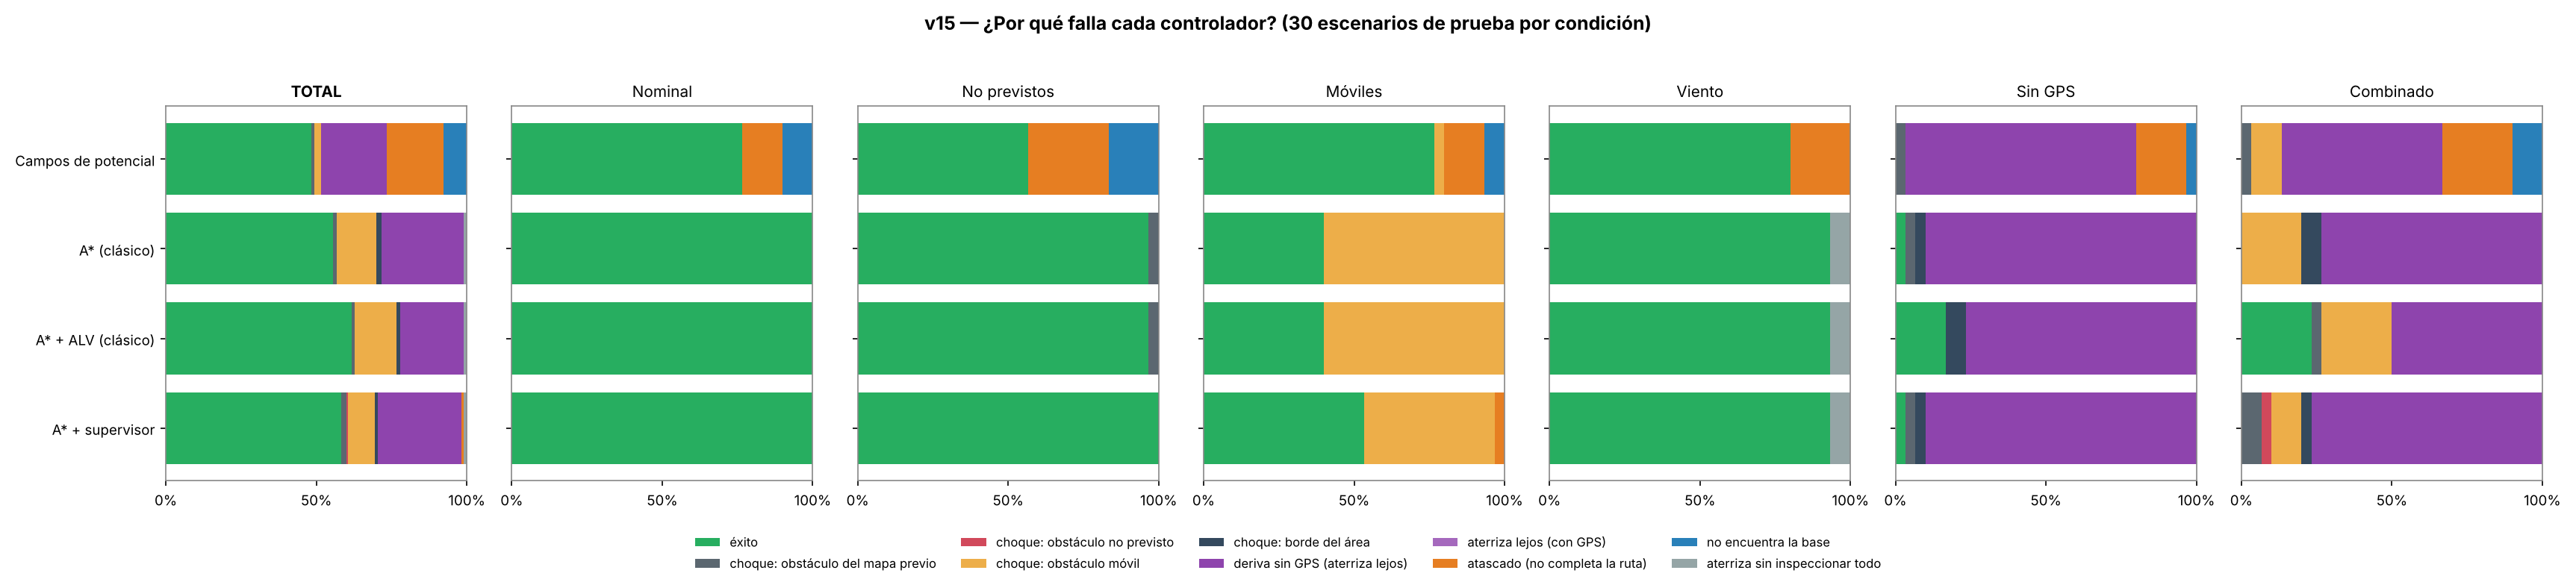
\includegraphics[width=0.95\textwidth]{v15_analisis_errores}
\caption{Causas de fallo por controlador y condición (\nfbEpisodiosPorCondicion{} escenarios
de prueba por condición).}
\label{fig:errores}
\end{figure*}
